\documentclass{standalone}
\usepackage{tikz}
\begin{document}
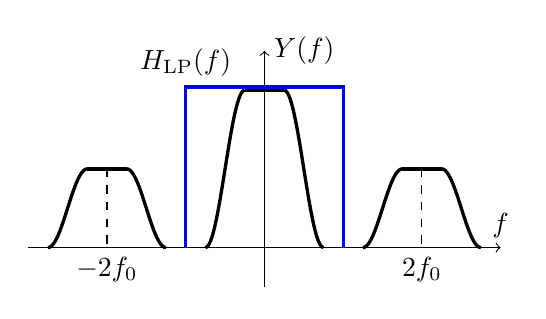
\begin{tikzpicture}[scale=2]
    \draw[->](0,-0.25)--(0,1.25)node[right]{$Y(f)$};
    \draw[->](-1.5,0)--(1.5,0)node[above]{$f$};

    
    \draw[very thick,smooth, domain=-0.375:-0.125]plot(\x,{0.5*(1+cos(4*pi*(abs(\x)-1/8) r))});
    \draw[very thick,smooth, domain=0.125:0.375]plot(\x,{0.5*(1+cos(4*pi*(abs(\x)-1/8) r))});
    \draw[very thick](-0.125,1)--(0.125,1);


    \draw[very thick,smooth, domain=0.625:0.875]plot(\x,{0.25*(1+cos(4*pi*(abs(\x-1)-1/8) r))});
    \draw[very thick,smooth, domain=1.125:1.375]plot(\x,{0.25*(1+cos(4*pi*(abs(\x-1)-1/8) r))});
    \draw[very thick](0.875,0.5)--(1.125,0.5);

    \draw[very thick,smooth, domain=-0.625:-0.875]plot(\x,{0.25*(1+cos(4*pi*(abs(\x+1)-1/8) r))});
    \draw[very thick,smooth, domain=-1.125:-1.375]plot(\x,{0.25*(1+cos(4*pi*(abs(\x+1)-1/8) r))});
    \draw[very thick](-0.875,0.5)--(-1.125,0.5);

    \draw[very thick, blue](-0.5,0)--(-0.5,1.02)node[above,black]{$H_\mathrm{LP}(f)$}--(0.5,1.02)--(0.5,0);

    \draw[dashed](-1,0.5)--(-1,0)node[below]{$-2f_0$};
    \draw[dashed](1,0.5)--(1,0)node[below]{$2f_0$};
\end{tikzpicture}
\end{document}  